\section{Вероятностное пространство как математическая модель случайного эксперимента. Статистическая устойчивость.}
Предмет исследования теории вероятностей -- случайный эксперимент, он должен удовлетворять трём требованиям:

1) повторяемость -- должна быть возможность повторить этот эксперимент в тех же условиях много раз

2) отсутствие детерминистической регулярности -- у эксперимента должно быть несколько исходов

3) статистическая устойчивость частот -- если исследуем частоты события в двух разных сериях (серии экспериментов предполагают достаточно большое количество повторений), то получившиеся частоты должны быть близки.

Вероятностным пространством называется тройка $(\Omega, \mathcal{F}, p)$, где:

$\Omega$ -- пространство элементарных исходов

$\mathcal{F}$ -- множество событий

$p$ -- вероятностная мера


\begin{tabular}{c|c}
    Реальность & Математика \\
    \hline
    Результаты случайного эксперимента & $\omega_1, \ldots, \omega_n, \ldots$ 
    -- элементарные исходы \\
    \hline
    Событие & Событие $A \subset \Omega, \{ A \} = \mathcal{F}$ \\
    \hline
    Частота $N(A)$ & $p(A)$
    
\end{tabular}

Можно сказать, что вероятность -- идеализированное понятие частоты.

$p: \mathcal{F} \to [0, 1]$ удовлетворяет следующим условиям:

1) $p(\Omega) = 1$

2) $\forall A, B \in \mathcal{F} \ p(A \bigsqcup B) = p(A) + p(B)$.


\section{Дискретное вероятностное пространство. Классическая вероятность. Построение простейших вероятностных пространств. Элементы комбинаторики. Вероятность суммы событий.}
\Def

\textit{Дискретной вероятностной моделью} называется математическая модель, в которой $\Omega$ не более чем счётно. В этом случае $\mathcal{F} = 2^{\Omega}$.

Классическая теория вероятностей занимается математическими моделями дискретной теории вероятностей, в которой элементарные исходы равновероятны.

Пусть $\forall \omega \in \Omega \ p(\omega) = c$

Случай, когда $|\Omega| < \infty$.

$$
1 = p(\Omega) = p(\bigsqcup_{\omega \in \Omega} w) = 
\sum_{\omega \in \Omega} p(\omega) = c \cdot |\Omega|
$$

Получается, что $p(\omega) = \frac{1}{|\Omega|}$, а значит
$\forall A \in \mathcal{F} \ p(A) = \frac{|A|}{|\Omega|}$

Докажем, что в классической теории вероятностей не может быть счётной $\Omega$.

Возьмём произвольное конечное $B \in \mathcal{F}$ ($B \subset \Omega$).
Тогда

$$
1 = p(\Omega) \geq p(\bigsqcup_{\omega \in B} \omega) = 
\sum_{\omega \in B} p(\omega) = c \cdot |B|
$$

Так как $B$ можно выбирать сколь угодно большое, получаем противоречие с тем, что $c \cdot |B| \leq 1$.

\subsection*{Урновые схемы}

В урне находится $M$ белых шаров ($1, \ldots, M$) 
и $N - M$ чёрных шаров ($M + 1, \ldots, N$).

Вытаскиваем $n$ шаров.

1) С возвращением, с порядком

$\omega = (i_1, \ldots, i_n)$, $|\Omega| = N^n$.

2) Без возвращения, с порядком

$\omega = (i_1, \ldots, i_n)$, $|\Omega| = A_N^n$

3) Без возвращения, неупорядоченный выбор

$\omega = \{ i_1, \ldots, i_n \}$ 
или $\omega = (i_1, \ldots, i_n), i_1 < i_2 < \ldots < i_n$.

$|\Omega| = C_N^n$

4) С возвращением, неупорядоченный выбор

$\omega = (j_1, \ldots j_n)$, $j_i$ -- количество появлений $i$-го шара

$|\Omega| = C_{N + n - 1}^{N - 1} = C_{N + n - 1}^{n}$



\section{Геометрические вероятности. Задача “о встрече”.}
\Def \textbf{Геометрическая вероятность.}

Пусть $\Omega \subset \R^n$ и $p(A) = \frac{\mu(A)}{\mu(\Omega)}$

Много задач на геометрическую вероятность разобрано тут:

\url{http://www.mathprofi.ru/geometricheskoe_opredelenie_verojatnosti.html}

\textbf{Задача.}

Староста группы заметил, что семинарист приходит на занятия со случайным опозданием в пределах $15$ минут. При этом семинарист не пускает в аудиторию студентов, которые пришли после него позднее чем на $5$ минут. Староста же решил опоздать на семинар, но выбрал себе границу случайного опоздания всего в $10$ минут. Также он решила ждать семинариста не более $10$ минут после своего прихода, а если его не будет -- уйти. Какова вероятность того, что староста все же посетит семинар?

\underline{Решение}

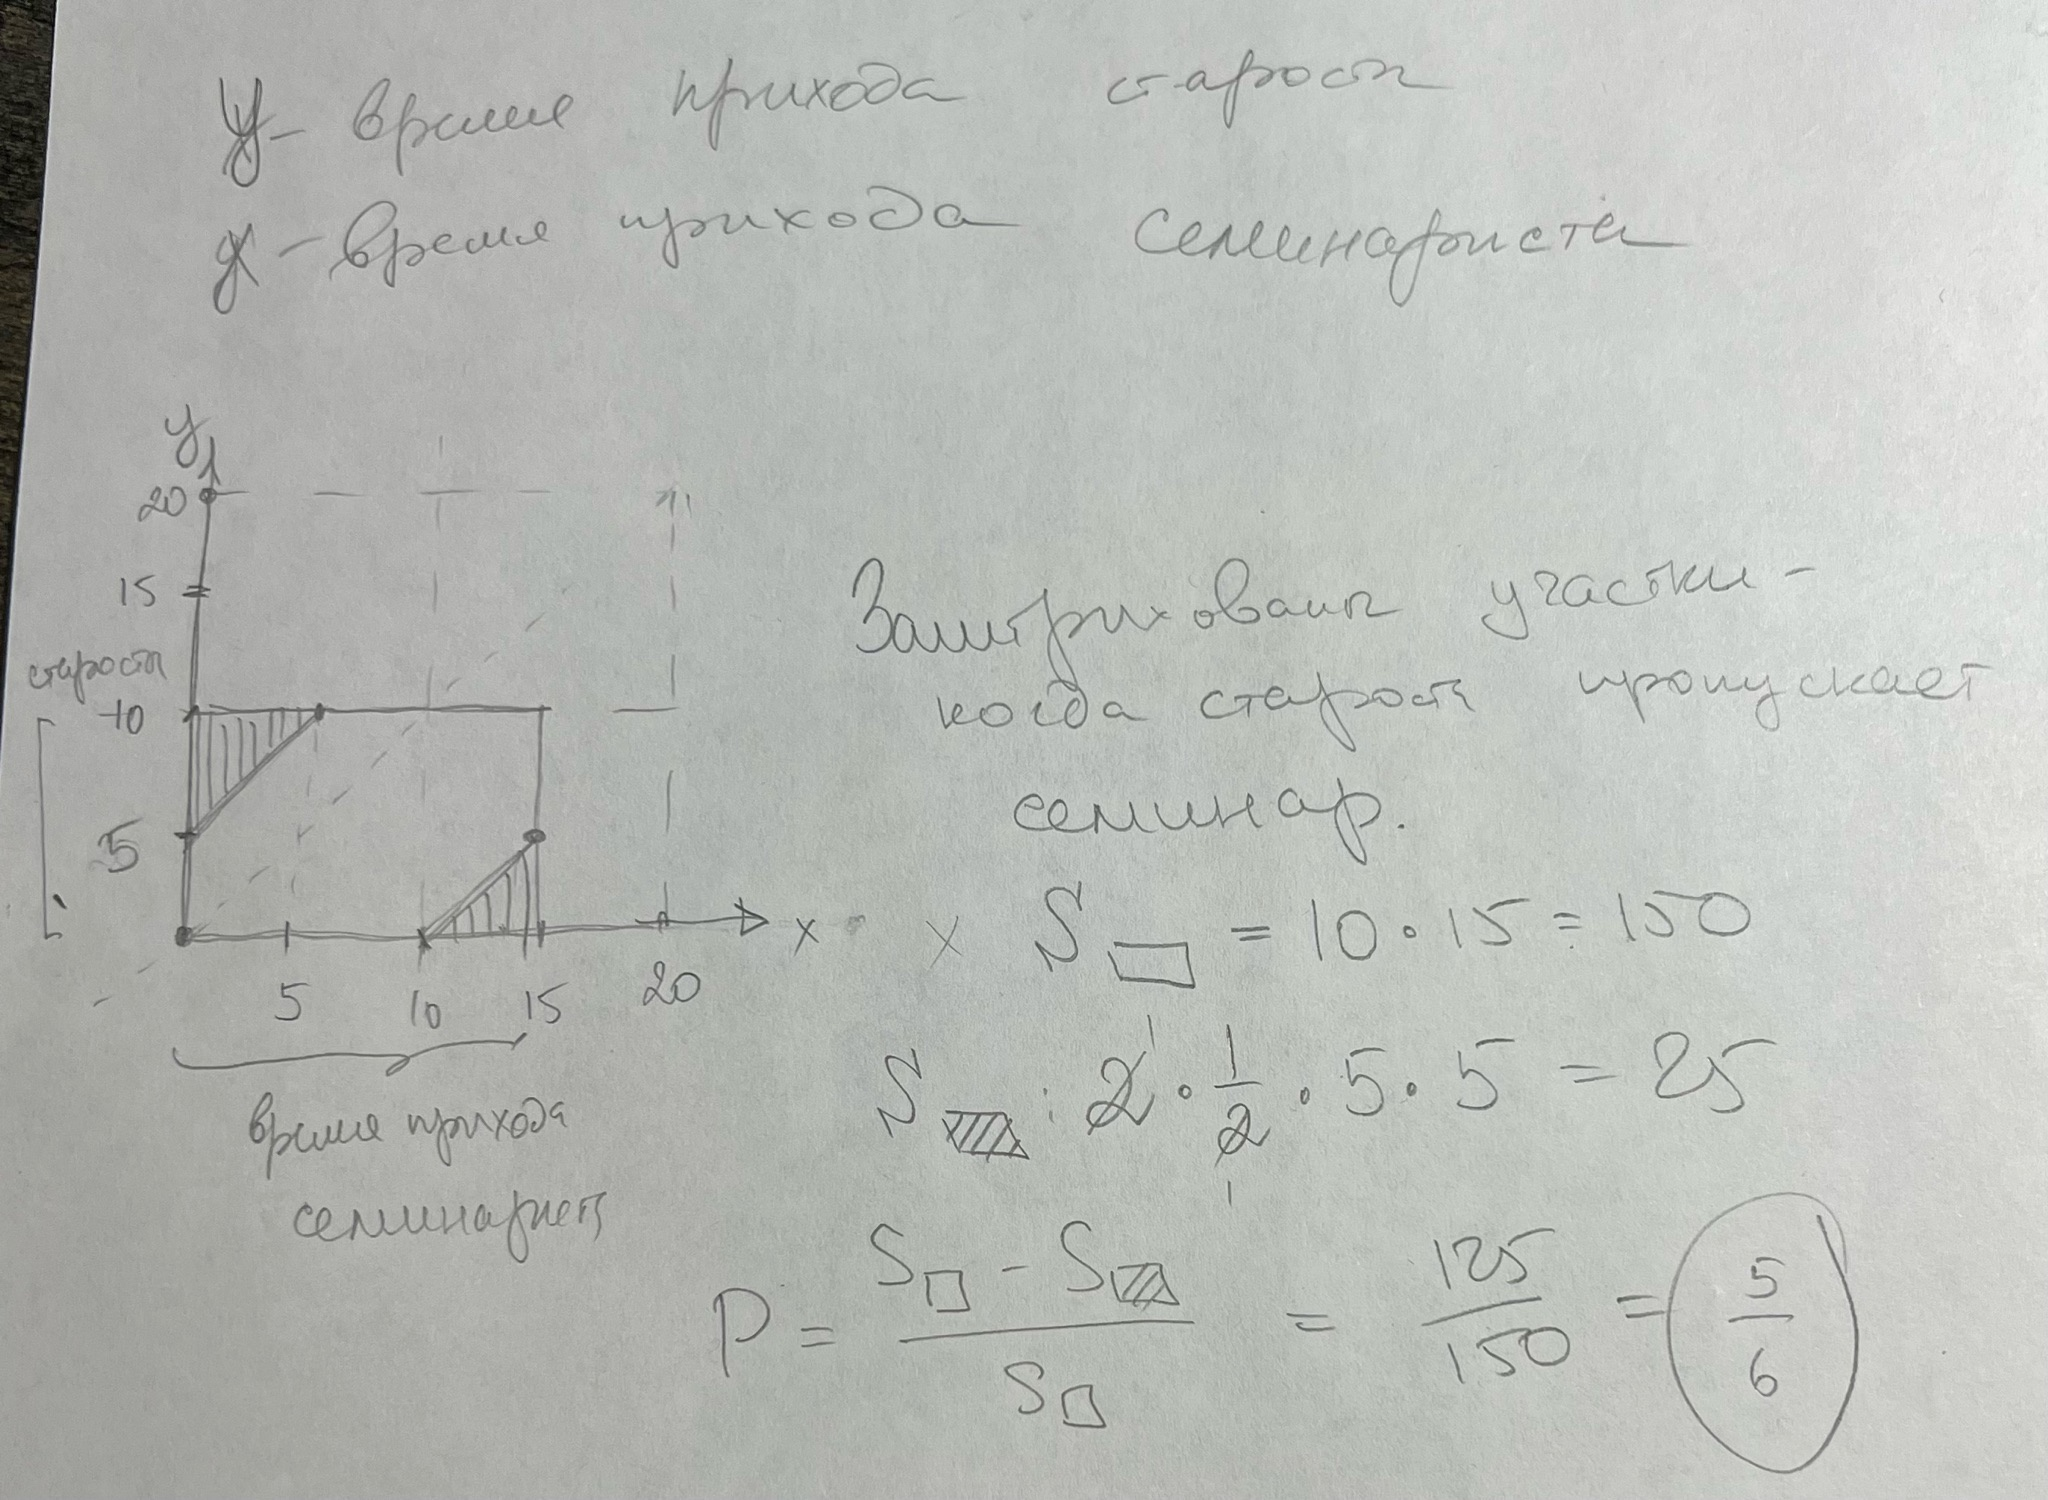
\includegraphics[width=12cm]{images/jetminded_solution.jpeg}
\newpage{}

\section{Условная вероятность. Формулы полной вероятности и Байеса.}

\Def \textit{Условная вероятность.} (Все еще живем в рамках вероятностного пространства $(\Omega, F, P)$ ).\\

\textbf{\textit{Сначала интуитивно:}}
Вероятность того, что событие $A$ произойдет при условии события $B$. Это значит, что мы теперь знаем, что событие $B$ произошло, и хотим в новых условиях посчитать вероятность того, что произойдет событие $A$.

На самом деле, это все такая же случайная вероятность, только теперь она случайна на немного другом множестве исходов (а именно, на множестве, когда произошло событие $B$, все остальные исходы нам недоступны).

\begin{minipage}[r]{0.15\linewidth} 
    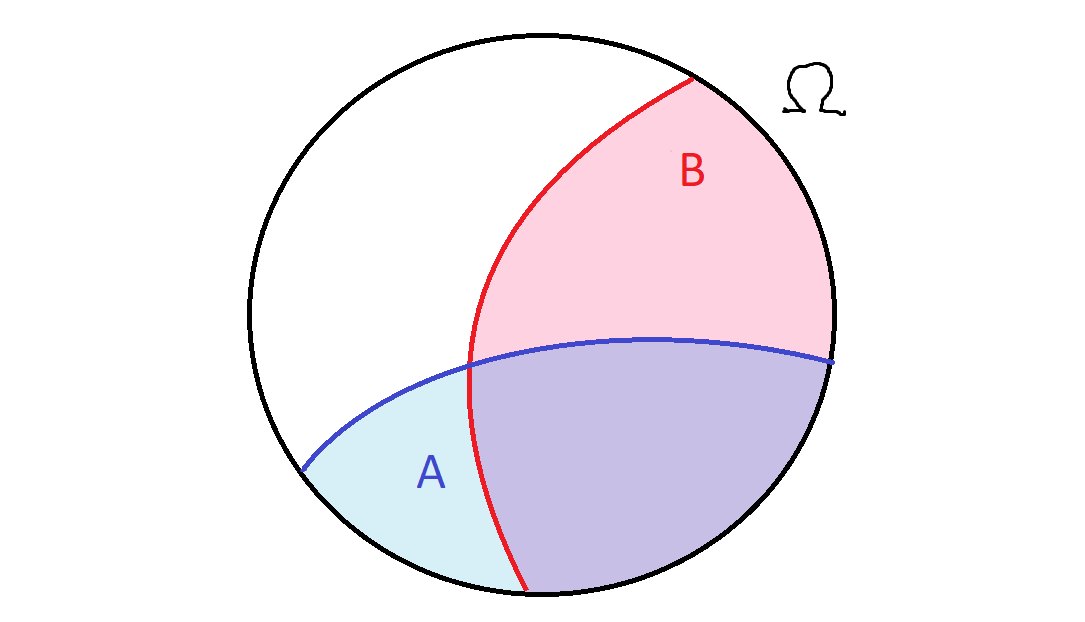
\includegraphics[width=2\linewidth]{images/4_1.png}
\end{minipage} \\

Если брать совсем классическую модель, то $P(A|B) = \frac{|A\cap B|}{|B|} = \frac{(\frac{|A\cap B|}{|\Omega|})}{(\frac{|B|}{|\Omega|})} = \frac{P(A\cap B)}{P(B)}$.

\textbf{\textit{Строгое определение}:}
Условная вероятность (в дискретной модели) события $A$ относительно события $B$, если $P(B) > 0$ определяется как $P(A|B) = \frac{P(A\cap B)}{P(B)}$

\Def \textit{Разбиением} называется такая (конечная или счетная) система событий $\{B_1, B_2, \dots \}$, что для любых различных $i$ и $j$ выполнено $B_i \cap B_j = \varnothing$ и $\cup B_i = \Omega$.\\

Пусть имеется разбиение $\{B_1, B_2, \dots \}$ с $P(B_i) > 0$. Тогда для любого события $A$ верна следующая формула:

\textbf{Формула полной вероятности:}

$P(A) = \sum\limits_{i}P(A|B_i)P(B_i)$

\Proof

$P(A) = P\Big(A \cap \Omega\Big) = P\Big(A \cap (\underset{i}{\bigsqcup} B_i)\Big) =  P\Big(\underset{i}{\bigsqcup} (A \cap B_i)\Big) = \sum\limits_i P(A \cap B_i) = \sum\limits_i P(A|B_i)P(B_i)$

\EndProof

Также, если имеется разбиение $\{B_1, B_2, \dots \}$ с $P(B_i) > 0$. Тогда для любого события $A$ верна еще и следующая формула:

\textbf{Формула Байеса}

$P(B_n|A) = \frac{P(A \cap B_n)}{P(A)} = \frac{P(A|B_n)P(B_n)}{\sum\limits_i P(A|B_i)P(B_i)}$

Пояснение на примере:

Пусть, в зависимости от того, насколько хорошо студент сдает сессию, родители могут оплатить ему путешествие. Чем хуже студент сессию сдает, тем меньше вероятность того, что ему могут оплатить поездку.

И вот мы хотим узнать, какова вероятность того, что студент на текущей сессии закрылся на отлично, если мы знаем, что он-таки отправился в путешествие.\\

\leftbar

Иван Генрихович называет такие вероятности умными словами \textit{апостериорная} -- $P(B_i|A)$ (эта вероятность на основе какого-то <<жизненного опыта>>, в данном случае -- поездка и есть тот самый опыт) и \textit{априорная} -- $P(B_i)$ (та, через которую мы ищем, для нее не нужен никакой <<жизненный опыт>>, в ней все понятно и последовательно, это знания, которые есть у нас изначально).
\endleftbar

\Note Если $A$ и $B$ -- множества, то запись $AB$ будем понимать как $A \cap B$

На лекциях была еще одна формула:

\textbf{Формула умножения вероятностей}

Если $P(A_1\dots A_n) \neq 0$, то ее можно вычислить по формуле

$P(A_1\dots A_n) = P(A_1) \cdot P(A_2|A_1) \cdot P(A_3|A_1A_2) \cdot \dots \cdot P(A_n|A_1\dots A_{n - 1})$

\Proof
$P(A_1\dots A_n) = P(A_1) \cdot P(A_2|A_1) \cdot P(A_3|A_1A_2) \cdot \dots \cdot P(A_n|A_1\dots A_{n - 1}) = P(A_1) \cdot \frac{P(A_1A_2)}{P(A_1)} \cdot \frac{P(A_1A_2A_3)}{P(A_1A_2)} \cdot \dots \cdot \frac{P(A_1\dots A_n)}{P(A_1\dots A_{n - 1})}$

Заметим, что все знаменатели у нас отличны от нуля, потому что эти вероятности не меньше, чем $P(A_1\dots A_n)$.

\EndProof


\section{Независимость событий, виды и взаимосвязь.}

\Def События $A$ и $B$ называются независимыми, если $P(AB) = P(A \cap B) = P(A)P(B)$.\\Обозначение:

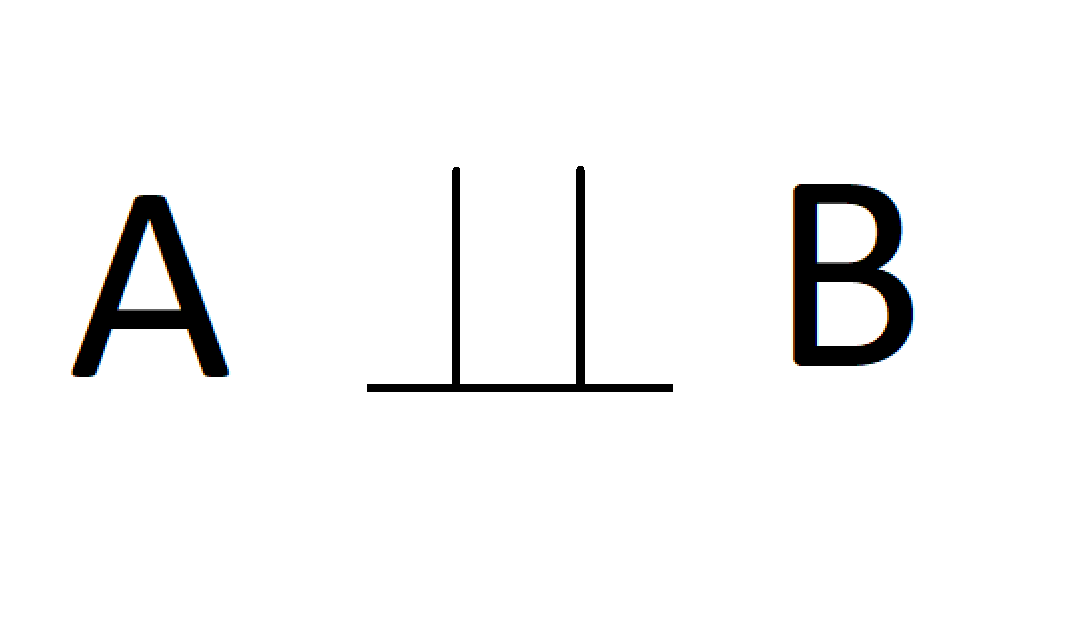
\includegraphics[width=0.1\linewidth]{images/5_1.png}

\textit{Откуда взялось определение:} идейно, хотим, чтобы событие $B$ никак не влияло на наступление события $A$, то есть хотим, чтобы $P(A|B) = P(A)$. Если расписать $P(A|B)$ получим $P(A) = \frac{P(A\cap B)}{P(B)}$, но такой формат записи чуть хуже -- тут мы запрещаем события нулевой вероятности, а, вообще говоря, можно считать, что они независимы со всеми, и их бы тоже надо учитывать. А еще мы хотим, чтобы формула была симметричной. Поэтому определение такое, как мы написали выше.

\Def $A_1, \dots, A_n \in F$ называются попарно независимыми, если $\forall i, j \leq n : A_i$ и $A_j$ независимы.

\Def События $A_1, \dots, A_n$ называются независимыми в совокупности, если для любых $i_1, \dots, i_k$ от $1$ до $n$ верно, что
$P(A_{i_1} \cap \dots \cap A_{i_k}) = P(A_{i_1}) \cdot$  $\dots$
$\cdot P(A_{i_k})$.

\Note Из независимости в совокупности следует попарная независимость, но не наоборот.

\Example Берем тетраэдр. Пусть первая грань красного цвета, вторая синего, третья зеленого, а четвертая -- всех трех цветов.
Каждая грань выпадает с вероятностью $\frac{1}{4}$, модель классическая.

Рассмотрим события $A_r, A_b, A_g$ -- выпадает грань, которая содержит соответствующий цвет.

Тогда мы знаем, что: 

$P(A_r) = P(A_b) = P(A_g) = \frac{1}{2}$, а еще $P(A_r \cap A_b) = P(A_r \cap A_g) = P(A_b \cap A_g) = \frac{1}{4}$, то есть попарная независимость у нас есть. Но независимости в совокупности здесь нет, потому что $P(A_r \cap A_b \cap A_g) = \frac{1}{4} \neq \frac{1}{8}$

\newpage{}

\section{Случайные величины. Независимость случайных величин. Распределение. Примеры. Математическое ожидание, дисперсия, ковариация, корреляция. Свойства.}

\Def Пусть дано дискретное вероятностное пространство $(\Omega, P)$. Дискретной случайной величиной $\xi$ называется произвольная функция $\xi 
: \Omega \to \mathbb{R}$.

\leftbar

\Def $\xi : \Omega \to \mathbb{R}$ называется случайной величиной, если $\forall x \in \mathbb{R} :  \xi^{-1}((-\infty; x]) \in \mathcal{F}$
\endleftbar

\Def Случайный величины $\xi$ и $\eta$ независимы, если $\forall x, y \in \mathbb{R}$ независимы события $(\xi = x)$ и $(\eta = y)$. Это определение работает только для дискретного случая. (Еще можно считать, что $x \in \xi(\Omega), y \in \eta(\Omega)$ т.к. 0 и 1 со всеми независимы).

\Def $\xi_1, \dots, \xi_n, \dots$  -- независимы в совокупности, если $\forall x_1, \forall x_2, \dots$ события $(\xi_1 = x_1), (\xi_2 = x_2), \dots$ независимы в совокупности.

\Def Распределением случайной величины $\xi$ -- это значения $\xi$ (а, точнее, $\xi(\Omega)$) и набор вероятностей $(p_1, \dots, p_n)$ таких, что $P(\xi = x_i) = p_i$

\leftbar

\Def Распределение случайной величины -- это вероятностная мера $P_{\xi}$ на $\mathbb{R}$, такая что $P_{\xi}(B) = P(\xi \in B)$ для любого борелевского подмножества прямой $B$.
\endleftbar

\Examples
\begin{enumerate}
    \item Бернуллиевское $\xi \sim Bern(p)$, тогда $P(\xi = 0) = 1 - p, P(\xi = 1) = p$
    \item Дискретное равномерное распределение $\xi \sim U[a, b]: P(\xi = k) = \frac{1}{b - a + 1}$
    \item Биномиальное распределение $\xi \sim Bin(n, p): P(\xi = k) = C_n^kp^k(1 - p)^{n - k}$
    \item Геометрическое $\xi \sim Geom(p): P(\xi = k) = p(1 - p)^k$ -- (кидаем монетку, орел на $k$ броске, до этого решка)
    \item Пуассоновское $\xi \sim Pois(\lambda): P(\xi = k) = \frac{\lambda^k}{k!}e^{-\lambda}$
\end{enumerate}


\Def Индикатором называется случайная величина, которая принимает значения $0$ или $1$. Индикатором события $A$ называется случайная величина $I_A(w) = \begin{cases} 
0,  & \mbox{если } w\not\in A\\
1,  & \mbox{если } w \in A 
\end{cases}$

Полезное свойство: $I_AI_B = I_{A\cap B}$

\Def Мат. ожидание (обобщение среднего значения) $E \xi = \sum\limits_{w \in \Omega} \xi(w)P(w)$

\Note Если $\Omega$ счетно, то нужно, чтобы ряд абсолютно сходился (потому что мы хотим, чтобы мат. ожидание не зависело от порядка нумерации элементарных исходов).

\leftbar

\Def Мат. ожидание $E \xi = \int\limits_{\Omega}\xi(w)dP$
\endleftbar

\textbf{Свойства:}

\begin{enumerate}
    \item \textit{Важная для подсчетов формула}: Пусть $x_1, \dots, x_n$ -- все возможные значения, принимаемые случайной величиной. Тогда $E\xi = \sum\limits_{w \in \Omega}\xi(w)P(w) = \sum\limits_{i=1}^nx_i \cdot \sum\limits_{\xi(w) = x_i}P(w) = \sum\limits_{i=1}^nx_iP(\xi = x_i)$
    
    \item $\xi \geq 0 \rightarrow E \xi \geq 0$ (слагаемые неотрицательные, поэтому сумма неотрицательна)
    \item \textit{Линейнойсть}: $\forall a \in \mathbb{R} : Ea\xi = a \cdot E \xi$ -- можно вынести множитель из суммы, отсюда и формула,
    $E(\xi + \eta) = E \xi + E \eta$
    
    Вообще говоря, складывать мы можем (поточечно) только те случайные величины, которые действиют из одного и того же вероятностного пространства.
    
    \Proof
    $E(\xi + \eta) = \sum\limits_{w \in \Omega}(\xi + \eta)(w)P(W) = \sum\limits_{w \in \Omega}\Big(\xi(w)P(w) + \eta(w)P(w)\Big) = \sum\limits_{w \in \Omega}\xi(w)P(w) + \sum\limits_{w \in \Omega}\eta(w)P(w) = E\xi + E\eta$
    \EndProof
    
    \item $\xi \geq \eta \rightarrow E\xi \geq E\eta$
    
    \Proof
    Следует из предыдущих двух пунктов: $\xi - \eta \geq 0 \rightarrow E(\xi - \eta) \geq 0$, а $E(\xi - \eta) = E\xi - E\eta \geq 0$
    \EndProof
    
    \item \textit{Неравенство треугольника} $|E\xi| \leq E|\xi|$
    
    \Proof
    $|\sum\limits_{w \in \Omega} \xi(w)P(w)| \leq \sum\limits_{w \in \Omega} |\xi(w)P(w)| = \sum\limits_{w \in \Omega} |\xi(w)|P(w) = E|\xi|$
    \EndProof
    
    \item \textit{Неравенство Коши-Буняковского}: $(E\xi\eta)^2 \leq E\xi^2E\eta^2$, причем равенство достигается тогда и только тогда, когда $\exists a, b \in \mathbb{R}, ab \neq 0 : a\xi + b\eta \stackrel{\mbox{п.н.}}{=} 0$ (в доказательстве вводится термин почти наверное)
    
    \Proof
    $\forall t \in \mathbb{R} : (t\xi - \eta)^2 \geq 0$
    
    $E(t\xi - \eta)^2 = E(t^2\xi^2 - 2t\xi\eta + \eta^2) = (E\xi^2)t^2 - (2E\xi\eta)t + E\eta^2 \geq 0$
    
    Т.к. это квадратный трехчлен от $t$, который всегда не меньше 0, то для его дискриминанта верно $(2E\xi\eta)^2 - 4E\xi^2E\eta^2 \leq 0$. Отсюда следует исходное неравенство.
    
    Анализируем, когда достигается равенство:
    
    \begin{enumerate}
        \item Вырожденный. Тогда $E\xi^2 = 0$, т.е. $\sum\limits_{w \in \Omega}\xi(w)^2P(w) = 0$, значит, $P(\xi = 0) = 1$.
        
        \Def $\xi \stackrel{\mbox{п.н.}}{=} 0$, если $P(\xi = 0) = 1$.
        
        Тогда $\xi + 0 \cdot \eta \stackrel{\mbox{п.н.}}{=} 0$
        
        \item $\exists t : E(t\xi - \eta)^2 = 0$, тогда $t\xi - \eta \stackrel{\mbox{п.н.}}{=} 0$.
    \end{enumerate}
    \EndProof
    
    \item $\forall A \in \mathcal{F} : EI_A = P(A)$.
    \Proof
    $EI_A = 1 \cdot P(I_A = 1) + 0 \cdot P(I_A = 0) = P(A)$    
    \EndProof
    
    \item Если $\xi$ и $\eta$ независимы, то $E\xi\eta = E\xi \cdot E\eta$.
    
    \Proof
    $E\xi\eta = \sum\limits_zzP(\xi\eta = z) = \sum\limits_zz\sum\limits_{(x, y) : xy = z}P(\xi = x, \eta = y) = \sum\limits_z\sum\limits_{(x, y) : xy = z}xyP(\xi = x)P(\eta = y) = \sum\limits_x\sum\limits_yxyP(\xi = x)P(\eta = y) = (\sum\limits_xxP(\xi = x))(\sum\limits_yyP(\eta = y))$
    \EndProof
    
    \Note Обратное неверно. 
    
    \Example $P(\xi = 1) = P(\xi = -1) = \frac{1}{4}, P(\xi = 0) = \frac{1}{2}, \eta = \xi^2$
    
    $E\xi = 0$, поэтому и $E\xi\eta = E\xi^3 = E\xi = 0$, $E\xi E\eta = 0$. Требуемое выполняется. Проверим теперь, что независимости нет. Для этого возьмем $x = y = 0$:
    
    $P(\xi = x, \eta = y) \neq P(\xi = x)P(\eta = y)$ т.к. $\frac{1}{2} \neq \frac{1}{2} \cdot \frac{1}{2}$
    
    \item $\phi : \mathbb{R} \to \mathbb{R}$
    
    $E\phi(\xi) = \sum\limits_{x \in \xi(\Omega)}\phi(x)P(\xi = x)$
    
    \Proof
    $E\phi(\xi) = \sum\limits_{w \in \Omega}\phi(\xi(w))P(w) = \sum\limits_{x \in \xi(\Omega)}\sum\limits_{w \in \Omega, \xi(w) = x}\phi(x)P(w) = \sum\limits_x\phi(x)\sum\limits_{w \in \Omega, \xi(w) = x}P(w) = \sum\limits_x\phi(x)P(\xi = x)$    
    \EndProof
\end{enumerate}


\Def Дисперсия $D \xi = E(\xi - E\xi)^2$

\textbf{Формула} $E(\xi - E\xi)^2 = E(\xi^2 - 2\xi E\xi + (E\xi)^2) = E\xi^2 - E(2\xi E\xi) + E(E\xi)^2 = E\xi^2 - 2(E\xi)^2 + (E\xi)^2 = E\xi^2 - (E\xi)^2$\\

\Def Стандартное отклонение $\sigma = \sqrt{D\xi}$

\Def Ковариацией $\xi, \eta$ называется $cov(\xi, \eta) = E(\xi - E\xi)(\eta - E\eta)$\\

\textbf{Формула} $cov(\xi, \eta) = E\xi\eta - E\xi E\eta$ (доказывается просто -- нужно раскрыть скобки и воспользоваться линейностью матожидания)

\textbf{Свойства}
\begin{enumerate}
    \item $cov(\xi, \xi) = D\xi$
    \item если $\xi$ и $\eta$ независимы, то $cov(\xi, \eta) = 0$ (по сути, это уже было нами доказано)
    \item $cov(\xi, \eta) = cov(\eta, \xi)$
    \item линейность по первому аргументу (а, значит, и по второму)
\end{enumerate}

\textbf{Теперь вернемся к свойствам дисперсии:}
\begin{enumerate}
    \item $D\xi \geq 0$, причем, $D\xi = 0 \Longleftrightarrow E(\xi - E\xi)^2 = 0 \Longleftrightarrow \xi - E\xi \stackrel{\mbox{п.н.}}{=} 0 \Longleftrightarrow \xi \stackrel{\mbox{п.н.}}{=} E\xi$, т.е. $\xi \stackrel{\mbox{п.н.}}{=} const$
    \item $D(a + b\xi) = b^2D\xi$
    \item если $\xi$ и $\eta$ независимы, то $D(\xi + \eta) = D\xi + D\eta$, естественным образом обобщается на попарно независимые независимые $\xi_1, \dots, \xi_n$: $D(\xi_1 + \dots + \xi_n) = D\xi_1 + \dots + D\xi_n$
    
    \Proof
    Докажем сразу для нескольких:
    $D(\xi_1 + \dots + \xi_n) = cov(\xi_1 + \dots + \xi_n, \xi_1 + \dots + \xi_n) = \sum\limits_{(i, j)}cov(\xi_i, \xi_j) = \sum\limits_{i=1}^ncov(\xi_i, \xi_i) + 2\sum\limits_{i<j}cov(\xi_i, \xi_j) = \sum\limits_{i=1}^nD\xi_i$
    \EndProof
\end{enumerate}

\Def Корреляцией $\xi$ и $\eta$ ($\xi \stackrel{\mbox{п.н.}}{\neq} const, \eta \stackrel{\mbox{п.н.}}{\neq} const$) называется 

$corr(\xi, \eta) = \frac{cov(\xi, \eta)}{\sqrt{D\xi}\sqrt{D\eta}}$.

Если $corr(\xi, \eta) = 0$, то $\xi$ и $\eta$ называются некоррелированными.\\

\Note Из независимости случайных величин следует $corr(\xi, \eta) = 0$, а в обратную сторону утверждение неверно.\\

\Statement $|corr(\xi, \eta)| \leq 1$, причем $corr(\xi, \eta) = \pm 1 \Longleftrightarrow \xi = a\eta + b$ для некоторых $a, b \in \mathbb{R}$

\Proof
Хотим показать, что $|cov(\xi, \eta)|^2 \leq D\xi \cdot D\eta$. Если расписать по определению, то получим просто частный случай неравенства Коши-Буняковского:

$(E(\xi - E\xi)(\eta - E\eta))^2 \leq E(\xi - E\xi)^2 \cdot E(\eta - E\eta)^2$, а равенство достигается, если $\exists a, b \in \mathbb{R} : a(\xi - E\xi) + b(\eta - E\eta) \stackrel{\mbox{п.н.}}{=} 0$. Также мы можем сказать, что $a \neq 0$, а поэтому на него можно поделить:

$\xi = -\frac{b}{a}\eta + \frac{b}{a}E\eta + E\xi$. Осталось обозначить соответствующий куски за искомые коэффициенты, и все получилось.
\EndProof

%\newpage{}

\section{Схема испытаний Бернулли. Математическая модель, теорема Пуассона.}
\par \textbf{Задача (подводка к схеме испытаний Бернулли):} Пусть у нас есть урна, в которой находятся $M$ белых и $N-M$ черных шаров. Вытаскиваем последовательно $n$ шаров с возвращением. Найти вероятность конкретной последовательности цветов.
\par \Solution Логично было бы ввести вероятностную модель, в которой элементарным исходом является последовательность цветов (последовательность из 0 и 1). Но она не является классической. Попробуем вывести ее из классической.
\par Будем считать все шары различными (занумеруем их: первые $M$ номеров соответствуют белым, остальные - чёрным). Тогда элементарный исход - последовательность номеров шаров длины $n$. Тогда $|\Omega|=N^n$. Пусть $A$ - событие соответствующее конкретной последовательности цветов, тогда $|A|=M^{n-\text{\#чёрных}}(N-M)^{\text{\#чёрных}}$, где \#чёрных - количество черных шаров в искомой последовательности. Если черный цвет мы обозначим как $\alpha_i=1$, а белый - $\alpha_i=0$, то \#чёрных$=\sum_{i=1}^N \alpha_i$. Тогда получаем $$P(A)=\frac{M^{n-\sum_{i=1}^N \alpha_i}(N-M)^{\sum_{i=1}^N \alpha_i}}{N^n}=\left(\frac{M}{N}\right)^{n-\sum_{i=1}^N \alpha_i}\left(\frac{N-M}{N}\right)^{\sum_{i=1}^N \alpha_i}$$
\par Если обозначим $\frac{N-M}{N}=p \in (0;1)$, то $\frac{M}{N}=1-p$ и $P(A)=p^{\sum_{i=1}^N \alpha_i}(1-p)^{n-\sum_{i=1}^N \alpha_i}$.
\par \textbf{Схема испытаний Бернулли:} Теперь можно ввести модель, которую мы хотели изначально: пусть $\omega=(\alpha_1, \ldots, \alpha_n), \alpha_i \in \{0,1\}$ - элементарный исход, $p(\omega)=p^{\sum_{i=1}^n \alpha_i}(1-p)^{n-\sum_{i=1}^n \alpha_i}$. Чтобы показать корректность нужно только проверить что $\sum_{\omega \in \Omega}p(\omega)=1$. Разобьём на суммы по количеству единиц в $\omega$
$$\sum_{\omega \in \Omega} p(\omega)=\sum_{k=0}^n \sum_{\omega: \: \sum_{i=1}^n\alpha_i=k} p^k (1-p)^{n-k}=\sum_{k=1}^n p^k(1-p)^{n-k} C_n^k=(p+1-p)^n=1$$

\par \textbf{Теорема Пуассона:} Пусть есть последовательность $\{p_n\}_{n=1}^\infty$, $p_n \in (0;1)$, $np_n \rightarrow \lambda$ при $n \rightarrow \infty$. Пусть $\{\xi_n\}_{n=1}^\infty$ - последовательность случайных величин, такая что $\xi_n \sim Bin(n, p_n)$. Тогда $$P(\xi_n=k)\rightarrow \frac{\lambda^k e^{-\lambda}}{k!}$$
\par \Proof $$P(\xi_n=k)=C_n^kp_n^k(1-p_n)^{n-k}=\frac{n(n-1)\ldots(n-k+1)}{k!}p_n^k\frac{(1-p_n)^n}{(1-p_n)^k}=$$
$$=\frac{1}{k!}(np_n)^k\frac{n(n-1)\ldots(n-k+1)}{n^k}\frac{1}{(1-p_n)^k}(1-p_n)^n$$
\par Так как $k$ - константа, то третий множитель стремится к единицы. Из условия на предел $np_n$ следует, что $p_n \rightarrow 0$ при $n \rightarrow \infty$, а значит четвертый множитель тоже стремится к 1. Второй множитель стремится к $\lambda^k$. Рассмотрим последний множитель.
$$(1-p_n)^n=((1-\frac{1}{1/p_n})^{1/p_n})^{np_n}\rightarrow e^{-\lambda}$$
\par Таким образом получаем искомое равенство. \EndProof
\newpage{}

\section{Неравенство Маркова и Чебышева. Закон больших чисел. Центральная предельная теорема (б/д).}

\par \textbf{Неравенство Маркова:} Пусть $\xi\geq 0$ - случайная величина, $a \in \R, a > 0$. Тогда $$P(\xi \geq a) \leq \frac{E\xi}{a}$$
\par \Proof Пусть $I$ - индикатор. Тогда $$E\xi=E(\xi I(\xi \geq a) + \xi I(\xi < a))=E(\xi I(\xi \geq a))+E(\xi I(\xi < a)) \geq E(\xi I(\xi \geq a)) \geq$$ $$\geq a E(I(\xi \geq a))=aP(\xi \geq a) \: \blacksquare$$

\par \textbf{Неравенство Чебышева:} $$\forall \varepsilon > 0 \: P(|\xi - E\xi| \geq \varepsilon)\leq \frac{D\xi}{\varepsilon^2}$$
\par \Proof Подставим в неравенство Маркова случайную величину $(\xi - E\xi)^2$ и $a=\varepsilon^2$. Получим
$$P((\xi-E\xi)^2 \geq \varepsilon^2) \leq \frac{E(\xi-E\xi)^2}{\varepsilon^2}$$
\par Это выражение равносильно условию теоремы \EndProof

\par \textbf{Закон больших чисел:} Пусть $\{\xi_i\}_{i=1}^\infty$ - последовательность независимых одинаково распределенных случайных величин и $\exists D\xi_1, a=E\xi_1$. Тогда $$\forall \varepsilon>0 \: P\left(\left|\frac{\xi_1+\ldots+\xi_n}{n}-a\right|>\varepsilon\right) \rightarrow 0$$
\par \Proof Подставим в неравенство Чебышева $\xi=\frac{\xi_1+\ldots+\xi_n}{n}$. Так как величины одинаково распределены, то матожидания всех $\xi_i$ равны и $E\xi=\frac{1}{n}\sum_{i=1}^n E\xi_i=a$
$$P(|\xi-E\xi|>\varepsilon) \leq \frac{D\xi}{\varepsilon^2}=\frac{D(\xi_1+\ldots+\xi_n)}{n^2 \varepsilon^2}$$
\par Так как величины независимы, то дисперсия суммы равна сумме дисперсий. Получаем
$$P(|\xi - E\xi| > \varepsilon)\leq \frac{n D\xi_1}{n^2\varepsilon^2} \rightarrow 0 \: \blacksquare$$

\par \Note В законе больших чисел можно ослабить условия на $\xi_i$: заменить независимость на некоррелируемость и одинаковую распределенность на условие $\sum_{i=1}^n D\xi_i =o(n^2)$.

\par \textbf{Центральная предельная теорема:} Пусть $\{\xi_i\}$ - последовательность независимых одинаково распределённых случайных величин, $\exists D\xi_1, E\xi_1=a, \sqrt{D\xi_1}=\sigma$. Тогда $\forall x, y \in \R \cup \{\pm \infty\}$ выполнено
$$P(x \leq \frac{\xi_1+\ldots+\xi_n-na}{\sqrt{n}\sigma}\leq y)\rightarrow \int_x^y \frac{1}{\sqrt{2\pi}}e^{-\frac{t^2}{2}}dt$$
\newpage{}